\subsection{Point of sail}
A sailboat can achive velocity by catching wind in the sail at different angles. This is called point of sail and the velocity is dependent on the dinghys displacement from the true wind direction, the wind experienced for a stationary object, where the velocity is a resultant of the force vector created by the wind depending on the alignemnt of the sail and the direction from where the wind is coming. There are five different states of point of sail that are divided into degrees away from the true wind origin. These are
\begin{labeling}{alligator}
\item [Luffing] (no propulsive force) angle between 0-30\degree
\item [Close-hauled] (lift) angle between 30-50\degree
\item [Beam reach] (lift) angle 90\degree
\item [Broad reach] (lift–drag) angle aound 135\degree
\item [Running] (drag) angle around 180\degree
\end{labeling}
and are represented in figure \ref{points-sail}. A sailor wants to prevent the sail from luffing when the sail starts to flap in the wind and no propulsive force is achived. When the dinghy is in the close-hauled and beam reach state the sail produces lift force that is produced from the avarage pressure differences on the windward and leeward side of the sail where the pressure is higher on the windward surface thus acting like a wing propelling the dinghy. When the dinghy is in the broad reach state both lift and also drag propells the dinghy. Drag acts like a parachute that that catches the wind and propelles the dinghy. The sideway force induced on the boat also introduces drift perpendicular to the relative bearing. This is counteracted by lowering a centerboard which also counteracts the dinghy from heeling.
\begin{figure}[H]
\centering
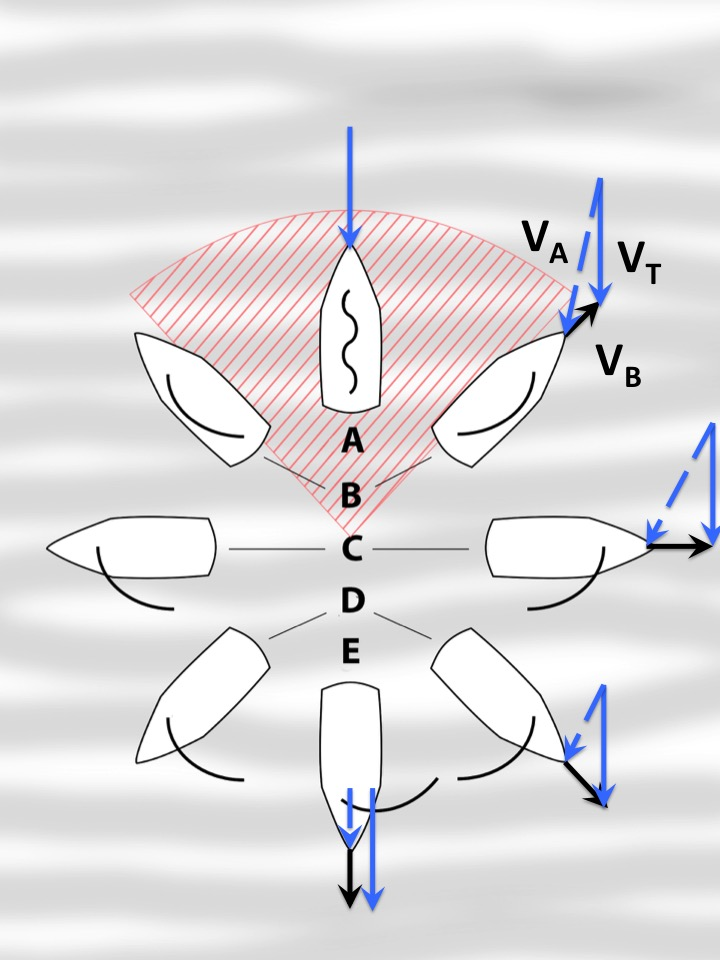
\includegraphics[width=0.6\textwidth]{Figures/Points_of_sail.jpg}
\caption{Points of sail}
\label{points-sail}
\end{figure}
\begin{figure}[H]
\centering
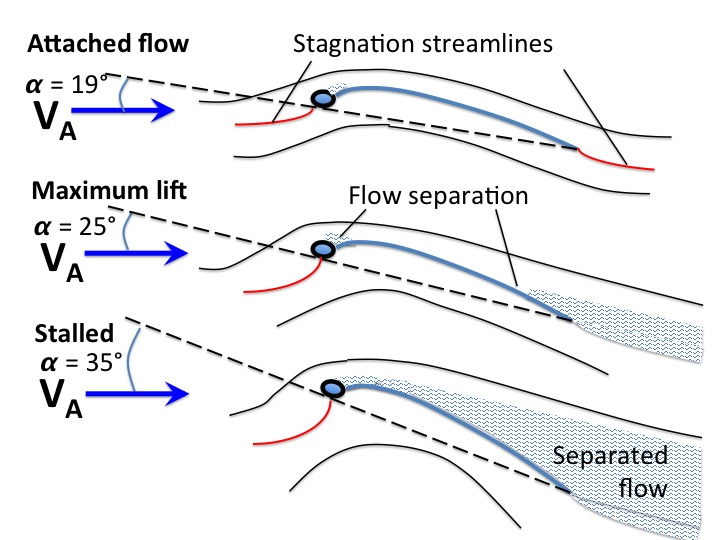
\includegraphics[width=0.6\textwidth]{Figures/max_lift.jpg}
\caption{Sail angles of attack}
\label{max_liftl}
\end{figure}
\subsection{Velocity}
The main goal in sailing is to maximize the efficiency at which the forces on the sail translates into velocity of the dinghy. A layman might expect that the fastest velocity is achived when the dinghy is parallel to the true wind, however this is not accurate. The apperent wind which is the wind experienced from the dingys perspective is what propells the dingy. When sailing paralell to the wind the dingys speed can never exceed the speed of the wind\cite{sail-force}. By sailing upwind close-halued the apperent wind is increased as the dingy accelerates until the drag from the water exceeds the forwad force created from the wind. To further increase the velocity of the dingy should not be heeling excessivly. This is to prevent the centerboard from acting as a rudder and changing the bearing and introducing more drag from the stern rudder when compansating for the bearing changes. As mentioned earlier the centerboard helps to counteract heeling but also the sailor can prevent this by hiking, leaning outside of the hull to alter the center of mass for the dinghy. Lastly when all other measures were taken the sailor must perform reefing and reducing the area of the sail and lowering the center of effort from the sails.